

Paātrinātāja sistēmas pamatā ir \Gls{fpga} ietvars, kas paredzēts IP kodolu savienošanas un programmatūras integrācijas
atvieglošanai, īpaši uz PCIe balstītās \Gls{fpga} ierīcēs. Tā kā pats straumēšanas konveijeru izveides ietvars 
promocijas darba netiek pilnībā apskatīts, šeit apkopotas tikai piedāvāto neiromorfo paplašinājumu izpratnei nepieciešamās koncepcijas.

Ietvars, kas parādīts \ref{fig:overall_arch}. attēlā, ietver sistēmas arhitektūras komponentu VHDL bibliotēku, kodola telpas
draiveri un lietotāja telpas API. Tas izveido konveijerizētu paātrinātāju, savienojot konveijerizētas \Gls{pu} ar AXI-Stream.
Lietotājam jānorāda tikai IP kodolu nosaukumu un parametru saraksts. Ietvars arī nodrošina reģistru kartēšanu, ļaujot
komponentus konfigurēt no draivera.

Datu pārsūtīšanai starp resursdatora skaitļošanas platformu, SDRAM un paātrinātāju izmanto AXI4-Full DMA moduļus. Lietotāja telpas API atbalsta modeļa ielādi paātrinātājā un atvieglo inferences izpildi.

\begin{figure}[!t]
  \centering
  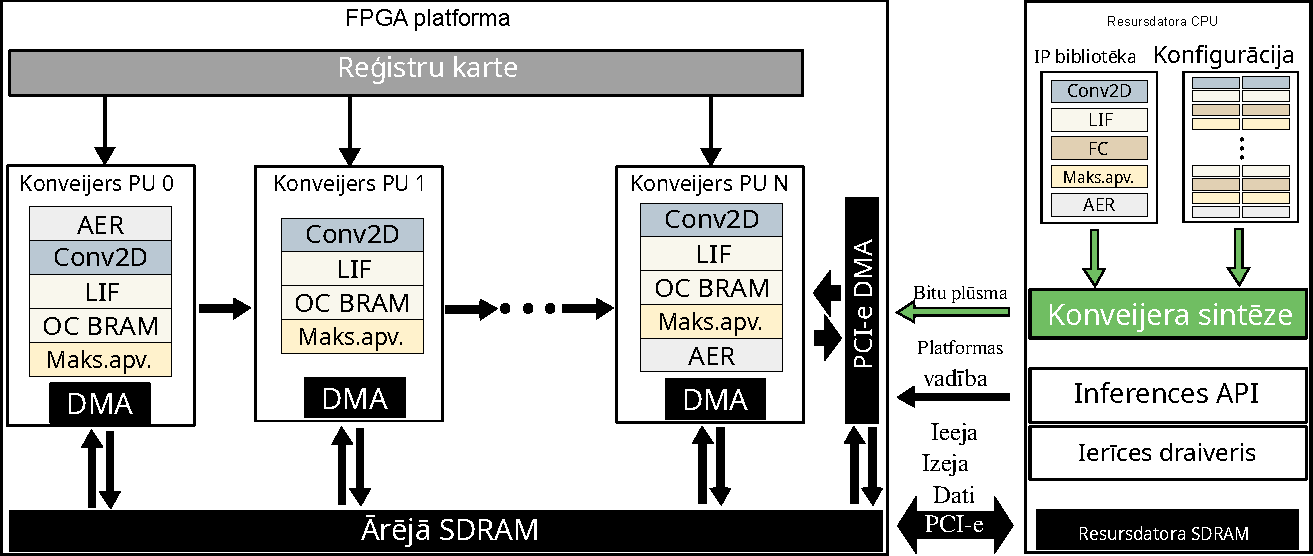
\includegraphics[width=0.75\linewidth]{fig/lv/snn_silhouse-v5.pdf}
  \caption{Automatizēta SNN paātrinātāja izveide heterogēnām skaitļošanas platformām.}
  \label{fig:overall_arch}
\end{figure}

Ietvars ir piemērots heterogēnām paātrinātāju sistēmām, kas CPU operācijām izmanto resursdatora skaitļošanas platformu un realizē \Gls{snn} inferenci PCIe \Gls{fpga} paplašināšanas kartēs. Tādēļ šajā darbā ietvars papildināts ar uz notikumiem balstītiem konvolūcijas, neironu, apvienošanas un impulsu kodēšanas apstrādes blokiem konveijerizētu neiromorfo sistēmu izveidei.

Turpmākajās sadaļās detalizēti aprakstīta katra \Gls{pu}.


